\documentclass[xcolor=table]{beamer}

% Get settings
\usepackage{mybeamer}

% Formalia
\title{\huge{Detektion af det gyldne snit i digitaliserede malerier}}
\subtitle{DIKU Bachelorprojekt 2009 -- 2010\\{\tiny Ulrik Bonde, Kasper Steenstrup og Morten Thorlund}}
\author{Ulrik Bonde}
\date{Vinter 2010}

\begin{document}

\begin{frame}
    \titlepage
\end{frame}

\section{Det gyldne snit}
\subsection*{}

\begin{frame}

    \frametitle{Division in Extreme and Mean Ratios}

    \begin{figure}[!h]
        \centering
        \begin{picture}(240,5)
            \put(0, 10){$A$}
            \put(3, -5){\line(0, 1){10}}

            \put(75, 10){$\varphi$}

            \put(144, 10){$C$}
            \put(147, -4){\line(0, 1){8}}

            \put(192, 10){$1$}

            \put(233, 10){$B$}
            \put(236, -5){\line(0, 1){10}}

            \put(3, 0){\line(1, 0){233}}
        \end{picture}
    \end{figure}

    \[
        \varphi = \frac{A\ C}{C\ B} = \frac{A\ B}{A\ C}
    \]
    \[
        \varphi = \frac{\varphi + 1}{\varphi}
    \]

    \begin{block}{Milestene}

        \begin{itemize}
            \item Kendt af Euklid ca. 300 f. Kr. som \emph{DEMR}.
            \item Luca Pacioli kaldte det for \emph{De Divina Proportione} i 1509.
            \item Navngivet \emph{der Goldener Schnitt} af Martin Ohm i 1835.
        \end{itemize}

    \end{block}

\end{frame}

% 3

\subsection*{}
\begin{frame}

    \frametitle{Hvor findes det gyldne snit?}

    \begin{block}{Generelle hypoteser}

        Det gyldne snit er:

        \begin{itemize}
            \item <1> at finde i naturen.
            \item <1> specielt æstetisk tiltalende.
            \item <1> anvendt i arkitektur.
            \item <1-2> brugt i kompositionen af mange malerier.
        \end{itemize}

    \end{block}

    \visible<2>{
        \centering\vspace{1em}
        \textbf{Vi vil gerne undersøge, om der findes noget \emph{interessant} i det gyldne snit i malerier.}
    }

\end{frame}


\section{Det gyldne snit i malerkunsten}

\subsection*{}
\begin{frame}

    \frametitle{Findes det gyldne snit i malerkunsten?}

    At undersøge om der findes noget interessant i det gyldne snit,
    rejser nogle vigtige spørgsmål.

    \hspace{8em}

    \begin{block}{Spørgsmål}

        \begin{itemize}
            \item Hvor \emph{er} det gyldne snit i et maleri?
            \item Hvad er \emph{interessant} i maleriet?
            \item Hvornår \emph{findes} noget i det gyldne snit?
        \end{itemize}

    \end{block}

\end{frame}

\subsection*{}
\begin{frame}

    \frametitle{Det gyldne snit i et maleri}

    \only<1>{
    \begin{center}
        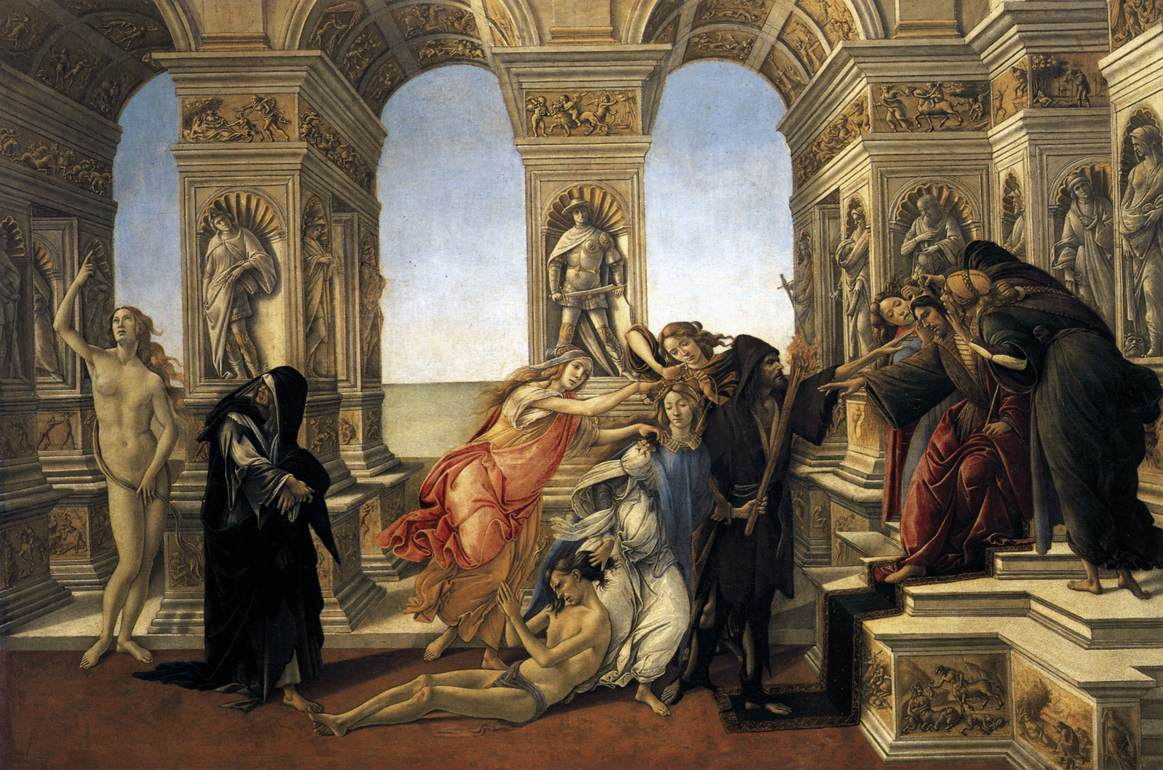
\includegraphics[width=1.00\textwidth]{billeder/10calumn.jpg}
    \end{center}
    }
    \only<2>{
    \begin{center}
        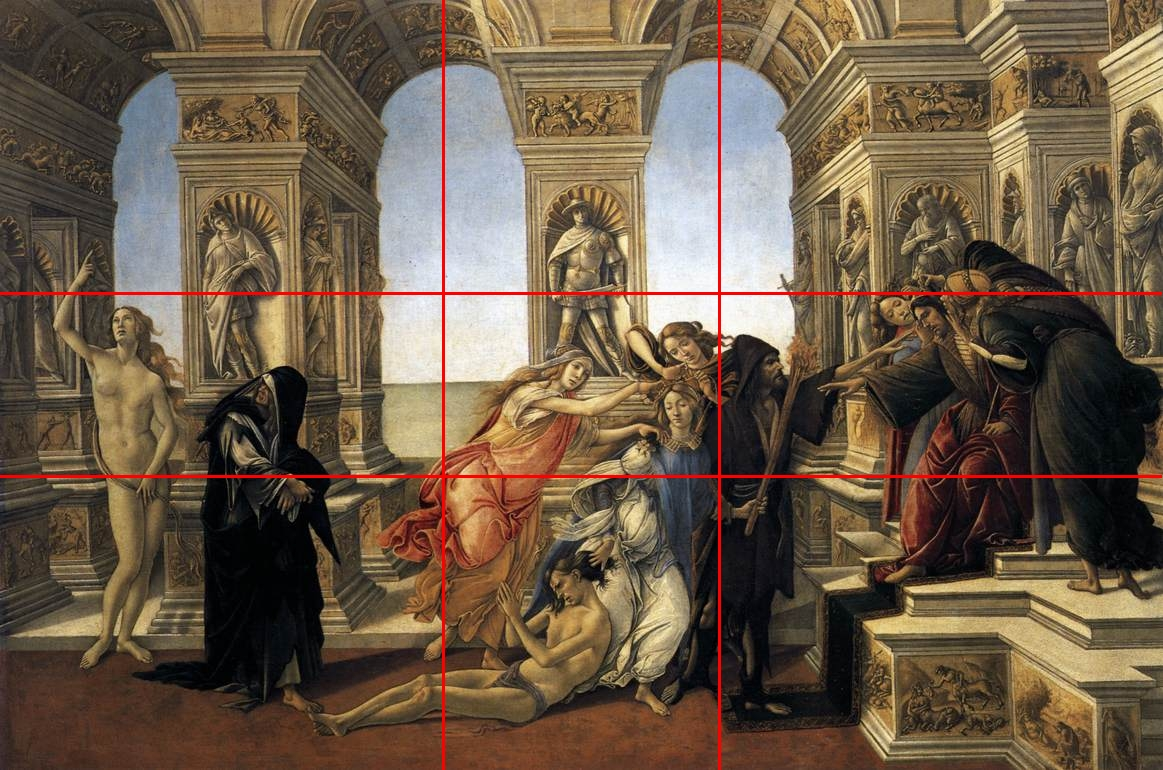
\includegraphics[width=1.00\textwidth]{billeder/10calumn_cut.jpg}
    \end{center}
    }

\end{frame}

\subsection*{}
\begin{frame}

    \frametitle{Hvad er interessant?}

    \only<1>{
    \begin{center}
        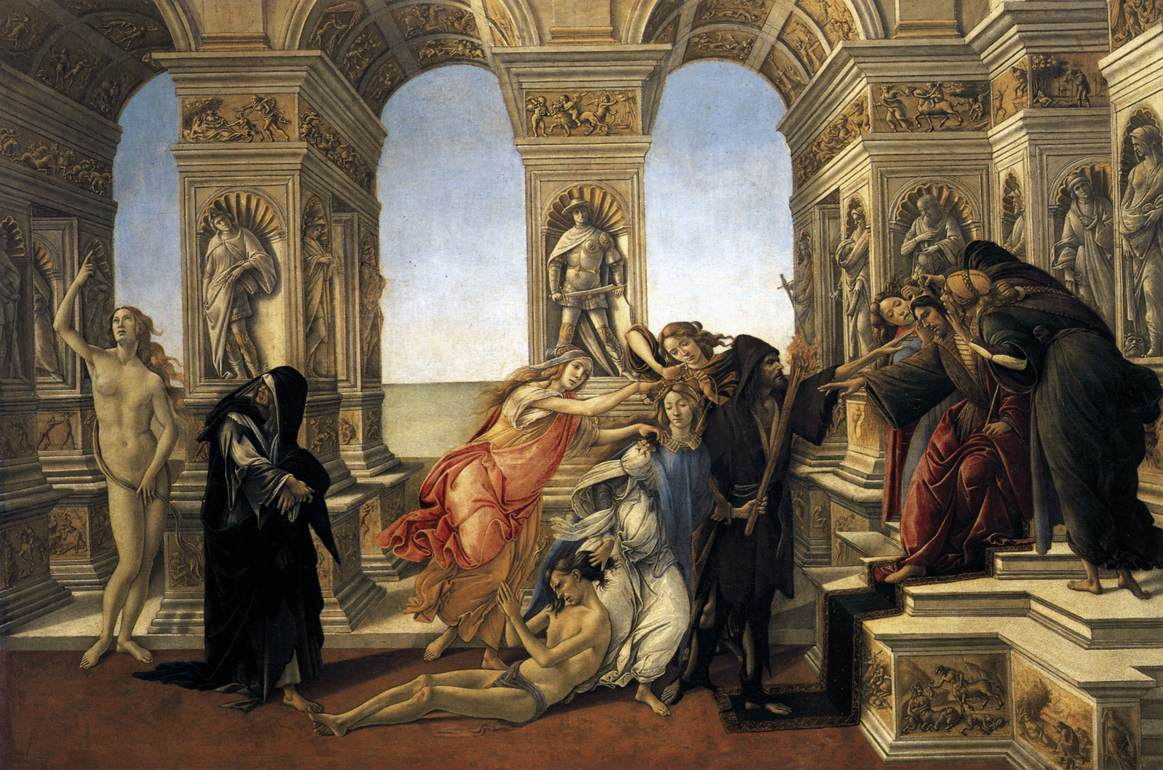
\includegraphics[width=1.00\textwidth]{billeder/10calumn.jpg}
    \end{center}
    }

    \only<2>{
    \begin{center}
        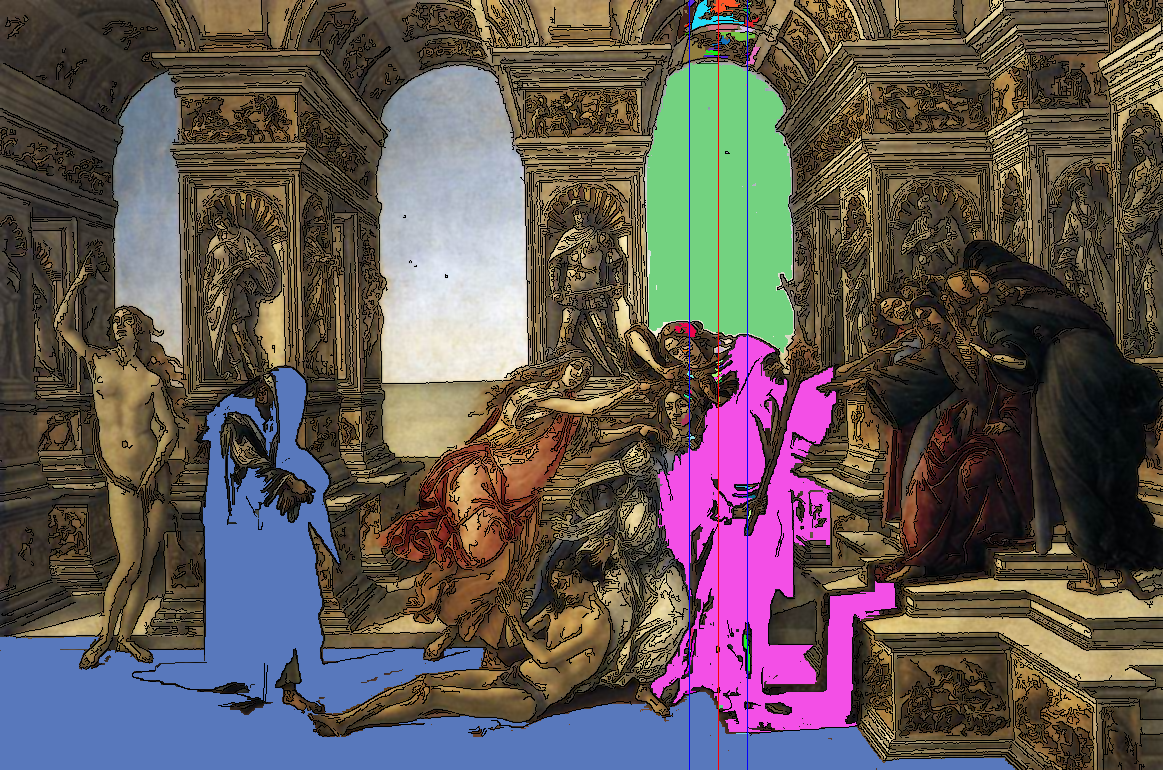
\includegraphics[width=1.00\textwidth]{billeder/10calumn_blobs}
    \end{center}
    }

    \only<3>{
    \begin{definition}
        En \textbf{\alert{region}} er en sammenhængende, ensfarvet gruppe pixels i
        et billede.
    \end{definition}

    \begin{definition}
        For at en region kan betegnes som \textbf{\alert{interessant}}, skal den
        \begin{itemize}
            \item have et areal større end en tærskelværdi, der sættes i
                forhold til billedets størrelse
            \item have en masse større end en tærskelværdi, der ligeledes,
                sættes i forhold til billedets størrelse,
        \end{itemize}
    \end{definition}
    }

\end{frame}

\subsection*{}
\begin{frame}

    \frametitle{Regioner i det gyldne snit}

    To forskellige måder, at betragte en region liggende i et snit på:

    \begin{center}
        \rowcolors[]{1}{gray!20}{gray!10}
        \begin{tabular}{l|cc}
            & \pos{Positiv} & \neg{Negativ}\\\hline
            Naiv    & 
\includegraphics[width=0.18\textwidth]{billeder/pnaiv_nudvidet} & 
\includegraphics[width=0.18\textwidth]{billeder/pudvidet_nnaiv}\\
            Udvidet & 
\includegraphics[width=0.18\textwidth]{billeder/pudvidet_nnaiv} & 
\includegraphics[width=0.18\textwidth]{billeder/pnaiv_nudvidet}
        \end{tabular}
    \end{center}

    Binær klassifikation: En interessant region enten {\pos{ligger}} eller {\neg{ligger ikke}} i snittet.

\end{frame}

\subsection*{}
\begin{frame}

    \frametitle{Repræsentation af regioner}

    To måder at repræsentere regioner på.

    \begin{columns}[t]
        \column{0.4\textwidth}
        \begin{exampleblock}{Begrænsende rektangel}
            \centering
            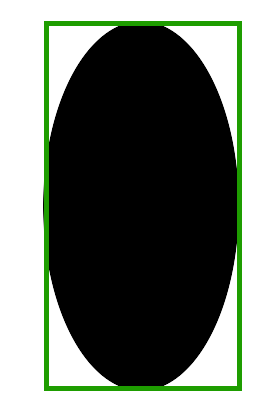
\includegraphics[width=0.6\textwidth]{billeder/blob_bbox}

            Bruges ved naiv bedømmelse
        \end{exampleblock}

        \column{0.4\textwidth}
        \begin{exampleblock}{Gitter}
            \centering
            
\includegraphics[width=0.6\textwidth]{billeder/blob_grid}

            Bruges ved udvidet bedømmelse
        \end{exampleblock}
    \end{columns}

\end{frame}

\subsection*{}
\begin{frame}

    \frametitle{Bedømmelse i praksis}

    \only<1>{
    Resultat fra de to metoder.

    \begin{columns}[t]
        \column{0.5\textwidth}
        \begin{exampleblock}{Naiv}
            \centering
            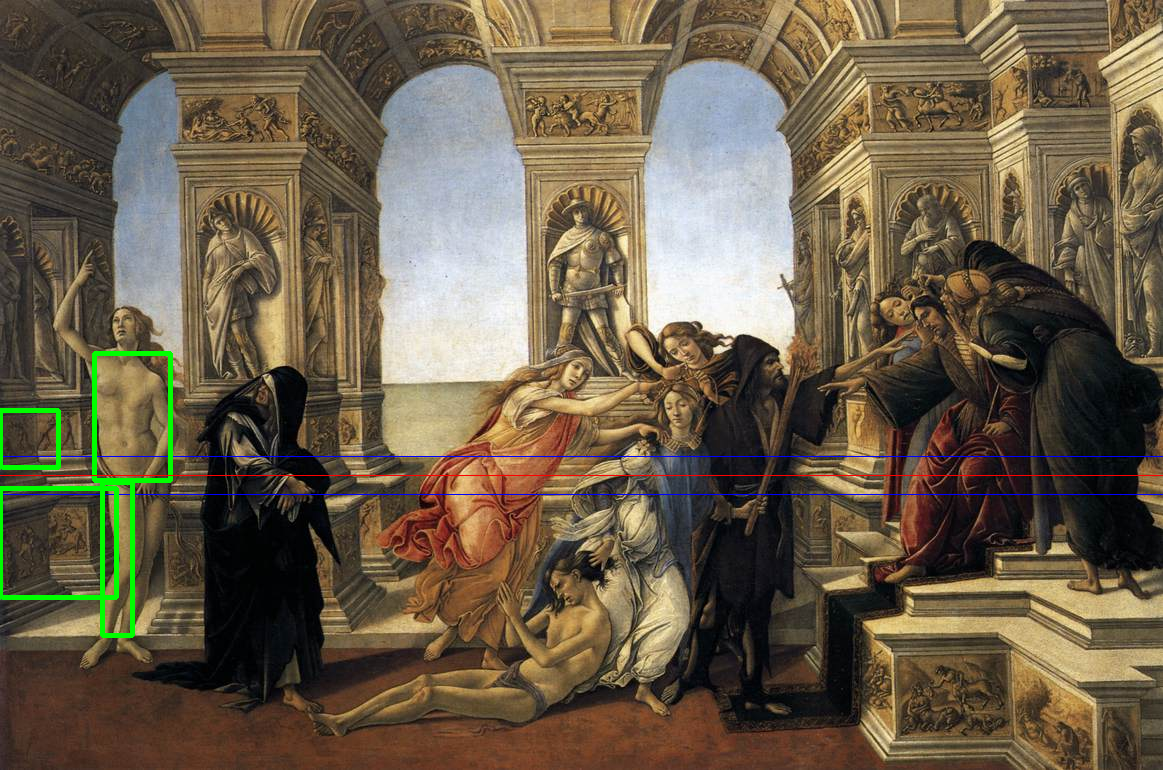
\includegraphics[width=1.0\textwidth]{billeder/10calumn_box_naive}
        \end{exampleblock}

        \column{0.5\textwidth}
        \begin{exampleblock}{Udvidet}
            \centering
            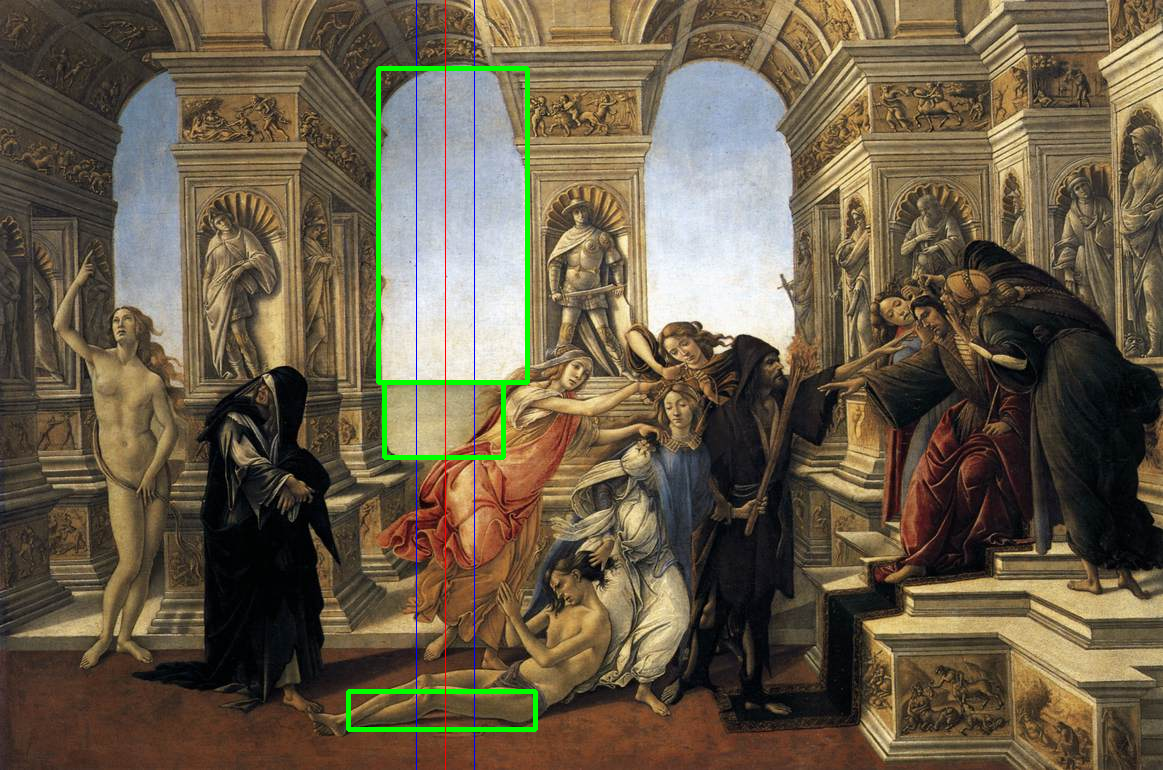
\includegraphics[width=1.0\textwidth]{billeder/10calumn_box_expanded}
        \end{exampleblock}
    \end{columns}
    }

    \only<2>{
        \begin{exampleblock}{Naiv}
            \centering
            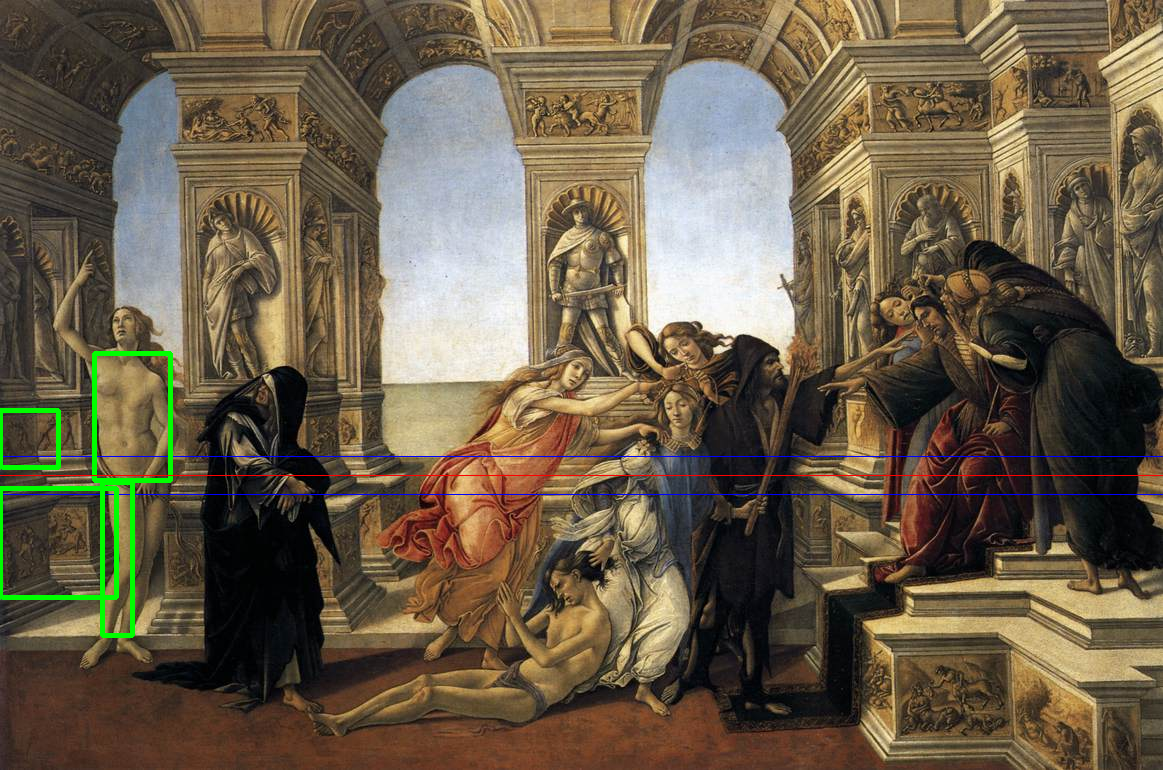
\includegraphics[width=0.85\textwidth]{billeder/10calumn_box_naive}
        \end{exampleblock}
    }
    \only<3>{
        \begin{exampleblock}{Udvidet}
            \centering
            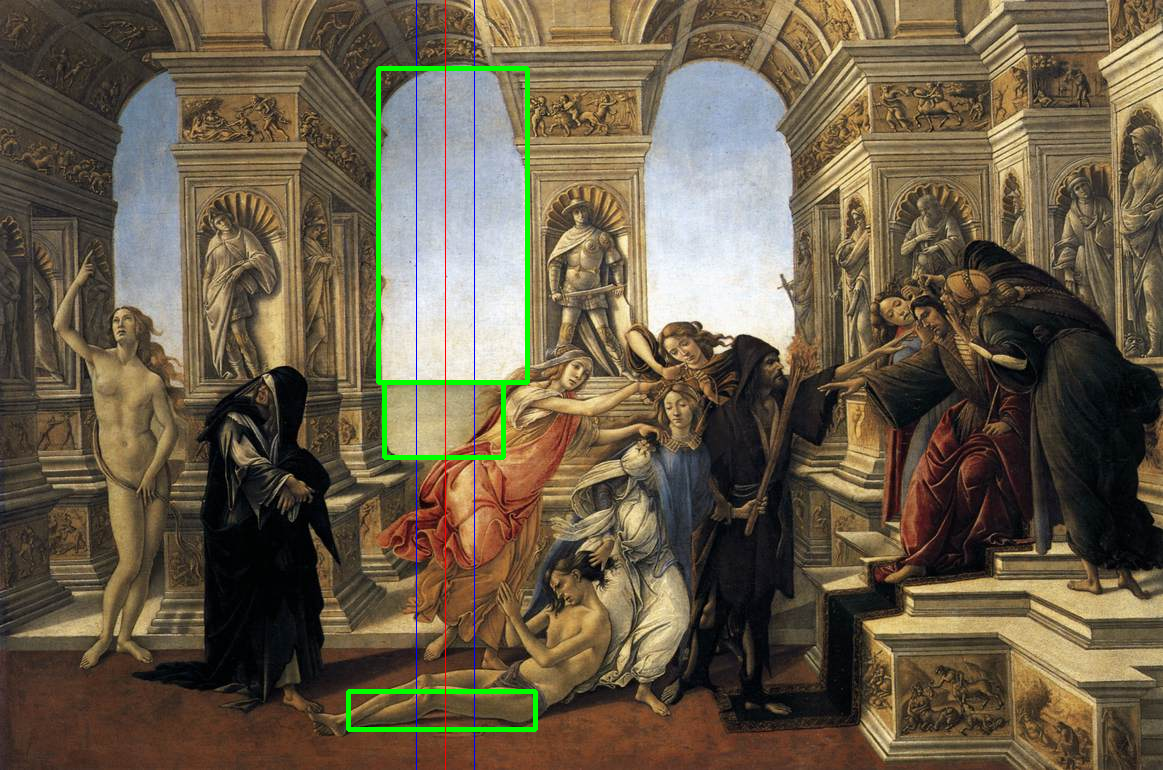
\includegraphics[width=0.85\textwidth]{billeder/10calumn_box_expanded}
        \end{exampleblock}
    }

\end{frame}

\section{Analyse på datasæt}
\subsection*{}
\begin{frame}

    \frametitle{Kørsler -- 40 snit undersøges}

    \begin{block}{Naiv kørsel}
        \begin{itemize}
            \item Kørt på 17.364 malerier.
            \item 14.375 brugbare resultater.
            \item \alert{Har duplikater af regioner.}
        \end{itemize}
    \end{block}

    \begin{block}{Udvidet kørsel}
        \begin{itemize}
            \item Ingen duplikater.
            \item Kørt på 608 malerier.
            \item \alert{524 brugbare resultater.}
        \end{itemize}
    \end{block}

\end{frame}

\subsection*{}
\begin{frame}

    \frametitle{Hypoteser}

    \begin{block}{Hypotese 1}
        Mere end \alert{$50\%$} af de analyserede malerier, har én eller flere
        interessante regioner i det gyldne snit.
    \end{block}

    \begin{block}{Hypotese 2}
        Antallet af interessante regioner, fundet i hvert af de fire snit
        tilknyttet snitratioen $\varPhi$, afviger ikke mere end \alert{$10\%$} fra
        hinanden.
    \end{block}

    \begin{block}{Hypotese 3}
        Mere end \alert{en tredjedel} malerierne har et lærred, hvis
        dimensioner er lig $\varphi\pm2,4\%$.
    \end{block}

\end{frame}

\subsection*{}
\begin{frame}

    \frametitle{Resultater fra analyser}

    \begin{block}{Resultat for hypotese 1\hspace{14em}\pos{Ikke afvist}}
        87,02 -- 91,43 \% af malerierne har mindst én region i det gyldne snit.
    \end{block}

    \begin{block}{Resultat for hypotese 2\hspace{16em}\neg{Afvist}}
        Antallet af regioner i hvert af de fire gyldne snit, afviger med 11,8 og 23,2 \% for hhv. naiv og udvidet kørsel.
    \end{block}

    \begin{block}{Resultat for hypotese 3\hspace{16em}\neg{Afvist}}
        Kun 4 \% af malerierne har et lærred opbygget efter det gyldne rektangel.
    \end{block}

\end{frame}

\subsection*{}
\begin{frame}

    \frametitle{Troværdige resultater?}

    \only<1>{
    Kan vi stole på resultaterne fra den naive analyse?

    \begin{columns}[t]
        \column{0.50\textwidth}
        \begin{block}{\neg{Bug}}
            \centering
            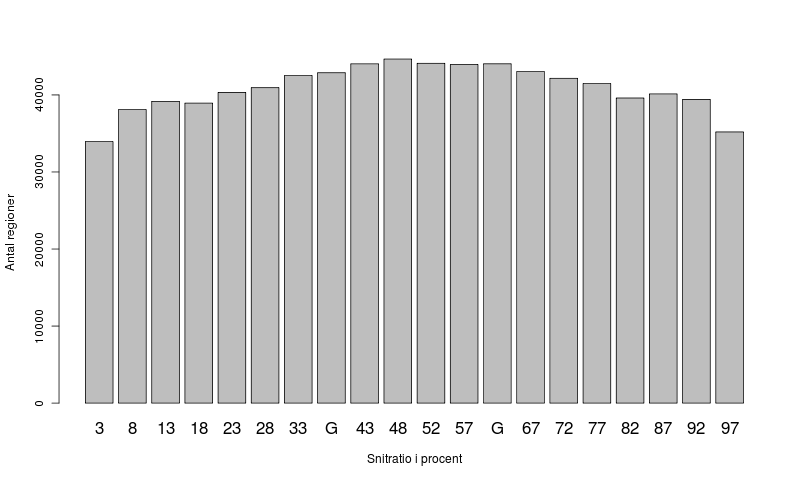
\includegraphics[width=0.80\textwidth]{billeder/cut0cut1eatsperratio}\\
            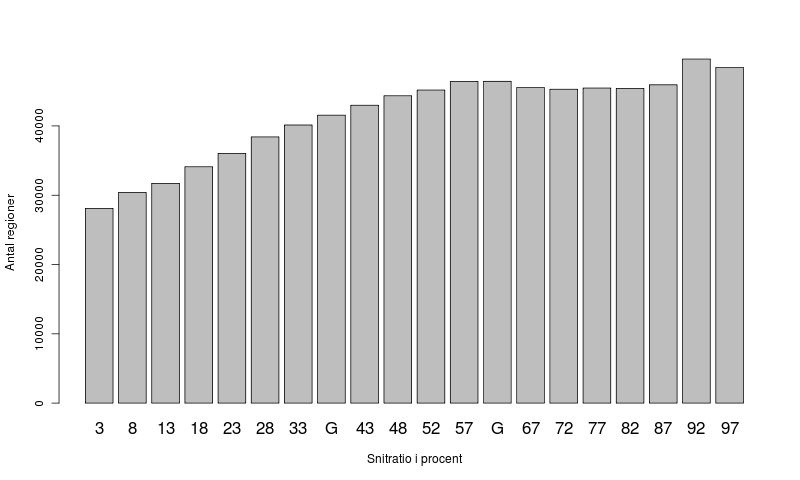
\includegraphics[width=0.80\textwidth]{billeder/cut2cut3eatsperratio}
        \end{block}


       \column{0.50\textwidth}
        \centering
        \begin{block}{\pos{Fix}}
            \centering
            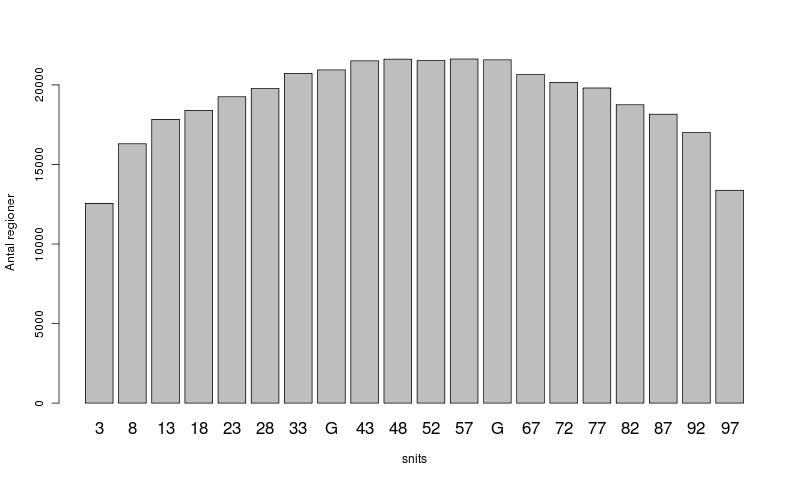
\includegraphics[width=0.80\textwidth]{billeder/cut0cut1eatsperrationNoBug}\\
            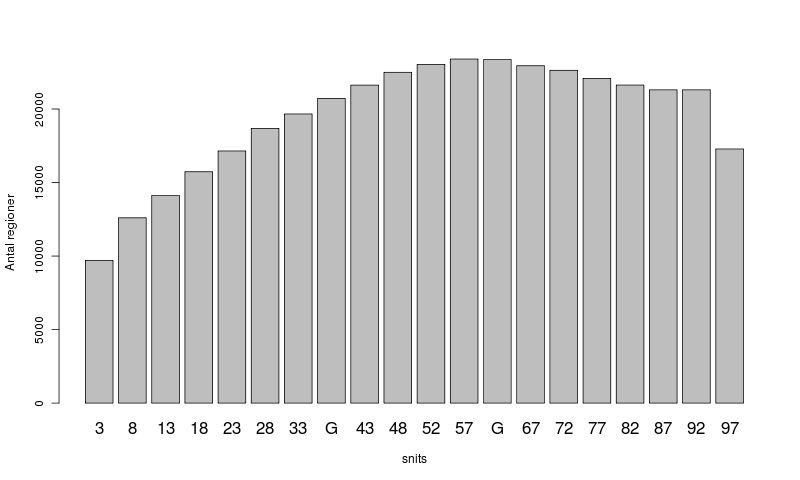
\includegraphics[width=0.80\textwidth]{billeder/cut2cut3eatsperrationNoBug}
        \end{block}

    \end{columns}
    }

    %\only<1>{
    %\begin{block}{Vertikale snit - \neg{Bug}}
    %    \centering
    %    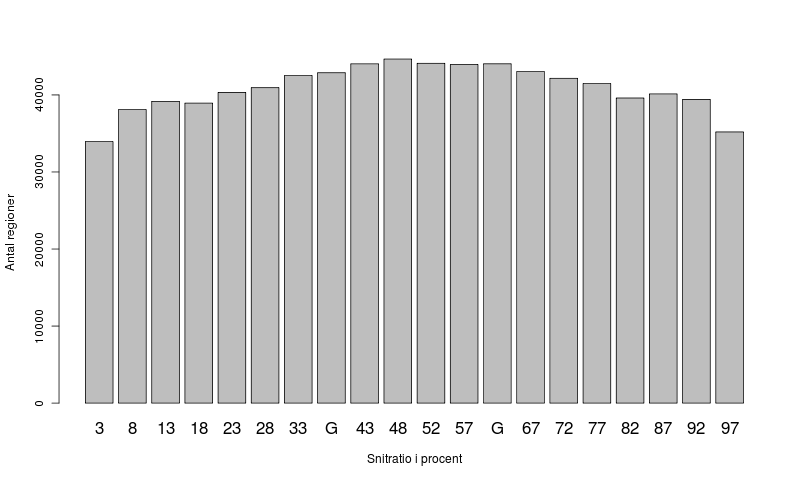
\includegraphics[width=0.8\textwidth]{billeder/cut0cut1eatsperratio}
    %\end{block}
    %}

    %\only<2>{
    %\begin{block}{Vertikale snit - \pos{Fix}}
    %    \centering
    %    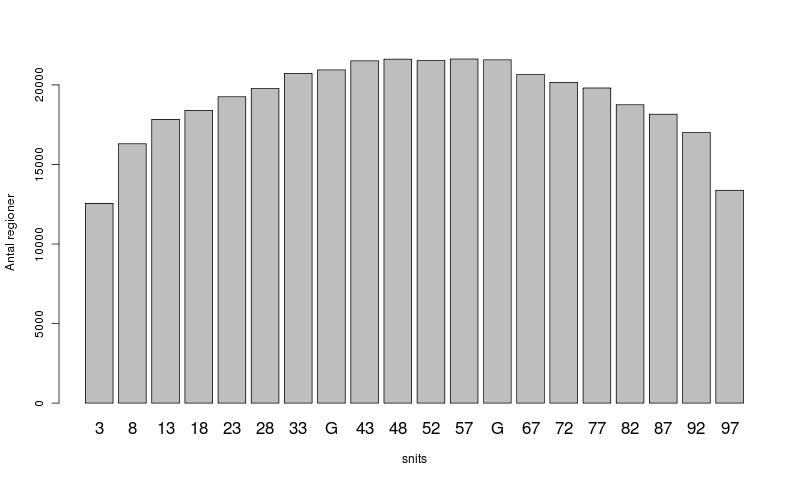
\includegraphics[width=0.8\textwidth]{billeder/cut0cut1eatsperrationNoBug}
    %\end{block}
    %}

    %\only<3>{
    %\begin{block}{Horisontale snit - \neg{Bug}}
    %    \centering
    %    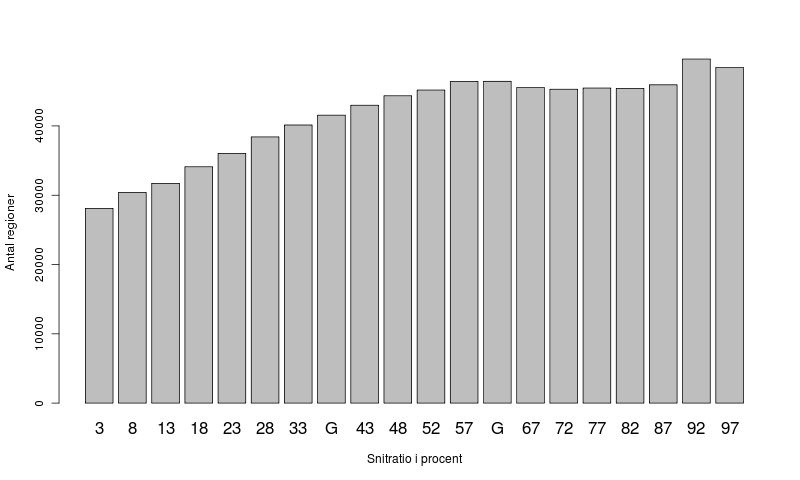
\includegraphics[width=0.8\textwidth]{billeder/cut2cut3eatsperratio}
    %\end{block}
    %}

    %\only<4>{
    %\begin{block}{Horisontale snit - \pos{Fix}}
    %    \centering
    %    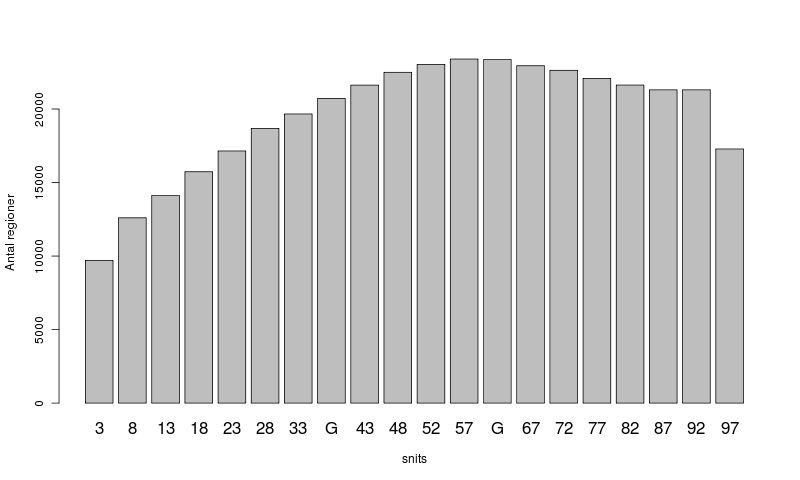
\includegraphics[width=0.8\textwidth]{billeder/cut2cut3eatsperrationNoBug}
    %\end{block}
    %}

    \only<2>{
    \begin{block}{Vurdering}
        \begin{itemize}
            \item Omkring en halvering i antal.
            \item Tendenserne viser samme mønster.
            \item Tendenserne er mere klare.
        \end{itemize}
    \end{block}
    }

\end{frame}

\subsection*{}
\begin{frame}

    \frametitle{Nye resultater}

    \begin{block}{Nyt resultat for hypotese 1\hspace{12em}\pos{Ikke afvist}}
        91,51 \% af malerierne har mindst én region i det gyldne snit.\\
    \end{block}

    \begin{block}{Nyt resultat for hypotese 2\hspace{14em}\neg{Afvist}}
        Maksimal afvigelse i antallet af regioner, i de fire gyldne snit, er 12,76 \%.
    \end{block}

    De nye resultater ændrer ikke på vores konklusioner.

\end{frame}

\section{Afslutning}
\subsection*{}
\begin{frame}

    \frametitle{Fortolkning}

    \begin{block}{Hvad har vi set?}
        \begin{itemize}
            \item<1-> Kunstnere foretrækker ikke at bruge et lærred med dimensioner som det gyldne rektangel.
            \item<2-> Det gyldne snit bruges ikke mere end andre snit. Specielt findes flere regioner i midten af maleriet.
            \item<3-> Antallet af regioner i det gyldne snit afhænger af kultur og stilperiode.
            \item<4-> Nogle gyldne snit foretrækkes frem for andre.
        \end{itemize}
    \end{block}

    \begin{block}{Mulige forbedringer}
        \begin{itemize}
            \item Bedre udtrækning af regioner.
            \item Mere målrettet definition på interessante regioner.
            \item Omkostning for regioner.
        \end{itemize}
    \end{block}

\end{frame}

\subsection*{}
\begin{frame}

    \only<1>{\frametitle{Tak}

    Spørgsmål

    }

    \only<2-4>{\frametitle{Udtrækning af regioner}}

    \only<2>{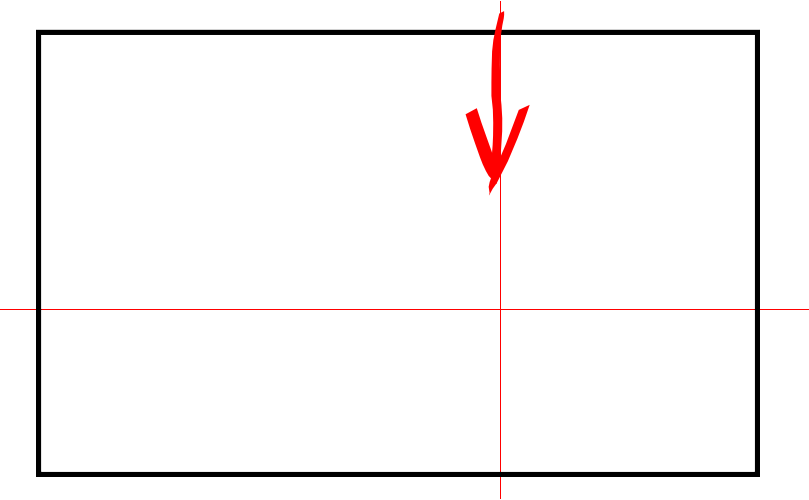
\includegraphics[width=\textwidth]{billeder/scan_direction_down}}
    \only<3>{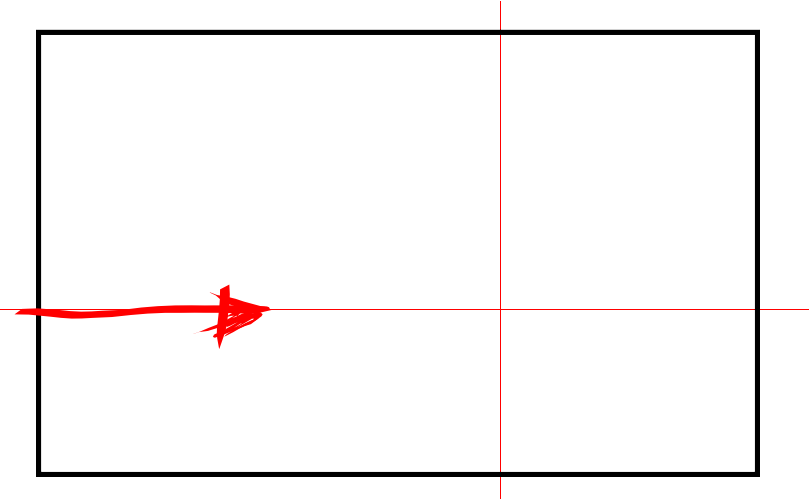
\includegraphics[width=\textwidth]{billeder/scan_direction_right}}
    \only<4>{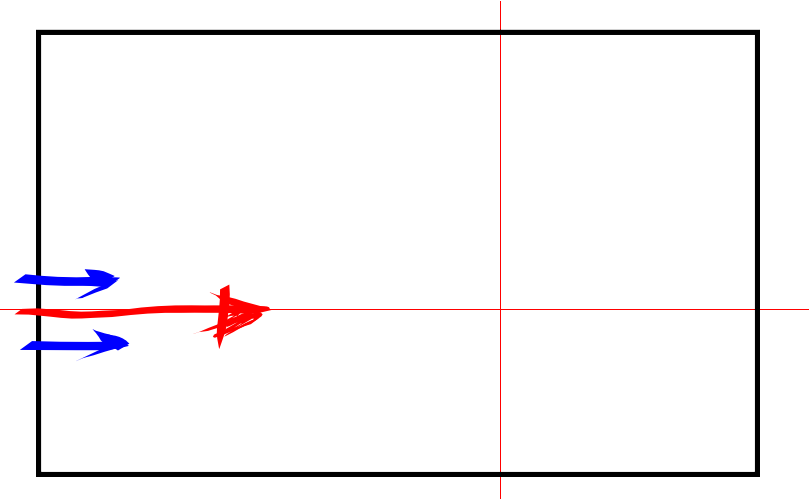
\includegraphics[width=\textwidth]{billeder/scan_direction_right_margin}}
    \only<5>{
        \setlength\fboxsep{0pt}
        \setlength\fboxrule{0.5pt}
        \fbox{
\includegraphics[width=\textwidth]{billeder/topographic_times}}
    }
    \only<6>{
    \frametitle{Datasæt}

    \begin{itemize}
        \item Primært renæssancemalerier af italienske kunstnere.
        \item Malerier kan være forkert beskåret eller opdelt.
    \end{itemize}
    }
    \only<7>{
    \frametitle{Regioner i de gyldne snit}

    \rowcolors[]{1}{gray!20}{gray!10}
    \begin{columns}[c]
        \column{0.5\textwidth}
        \begin{exampleblock}{Naiv \alert{med duplikater}}
            \begin{tabular}{r@{\ \ }p{7em}r}
                    & Regioner i $GS$ 0             &  $42.884$ \\
                $+$ & Regioner i $GS$ 1             &  $44.042$ \\
                $+$ & Regioner i \alert{$GS$ 2}             &  \alert{$46.432$} \\
                $+$ & Regioner i $GS$ 3             &  $41.547$ \\\hline
                & Alle $GS$       & $168.650$
            \end{tabular}
        \end{exampleblock}
        \column{0.5\textwidth}
        \begin{exampleblock}{Naiv uden duplikater}
            \begin{tabular}{r@{\ \ }p{7em}r}
                    & Regioner i $GS$ 0             &  $20.946$ \\
                $+$ & Regioner i $GS$ 1             &  $21.576$ \\
                $+$ & Regioner i \alert{$GS$ 2}             &  \alert{$23.357$} \\
                $+$ & Regioner i $GS$ 3             &  $20.713$ \\\hline
                & Alle $GS$       & $86.592$
            \end{tabular}
        \end{exampleblock}
    \end{columns}
    \begin{exampleblock}{Udvidet}
        \centering
        \rowcolors[]{1}{gray!20}{gray!10}
        \begin{tabular}{r@{\ \ }p{12em}r}
                & Regioner i $GS$ 0         &  $405$ \\
            $+$ & Regioner i $GS$ 1         &  $421$ \\
            $+$ & Regioner i \alert{$GS$ 2}         &  \alert{$499$} \\
            $+$ & Regioner i $GS$ 3         &  $492$ \\\hline
            & Alle $GS$   & $1.817$
        \end{tabular}
    \end{exampleblock}
    }

    \only<8>{
    \frametitle{Antal billeder mod antal regioner -- \alert{Bug}}

    \centering
    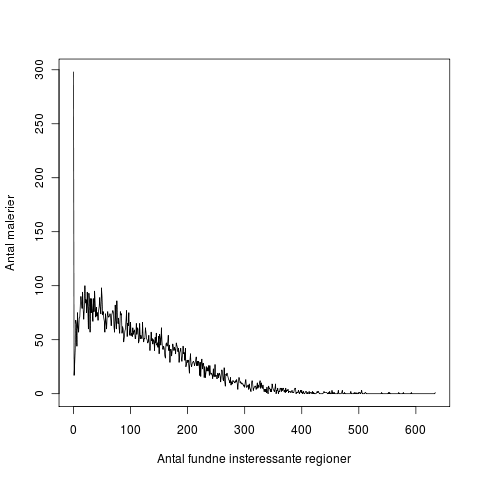
\includegraphics[width=0.65\textwidth]{billeder/totalregions_var}
    }

    \only<9>{
    \frametitle{Antal billeder mod antal regioner -- \pos{Fix}}

    \centering
    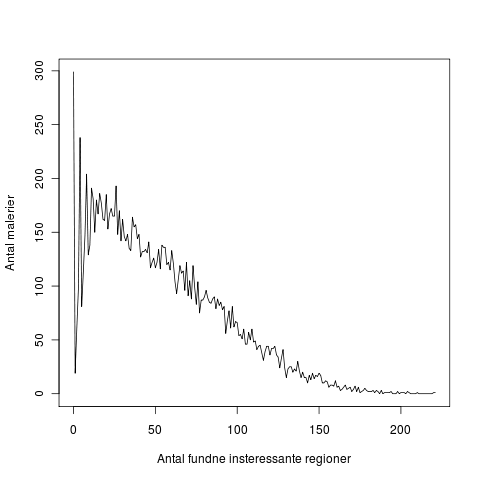
\includegraphics[width=0.65\textwidth]{billeder/totalregions_var_ny}
    }

    \only<10>{

    \frametitle{40 snit i maleriet}

    \begin{center}
        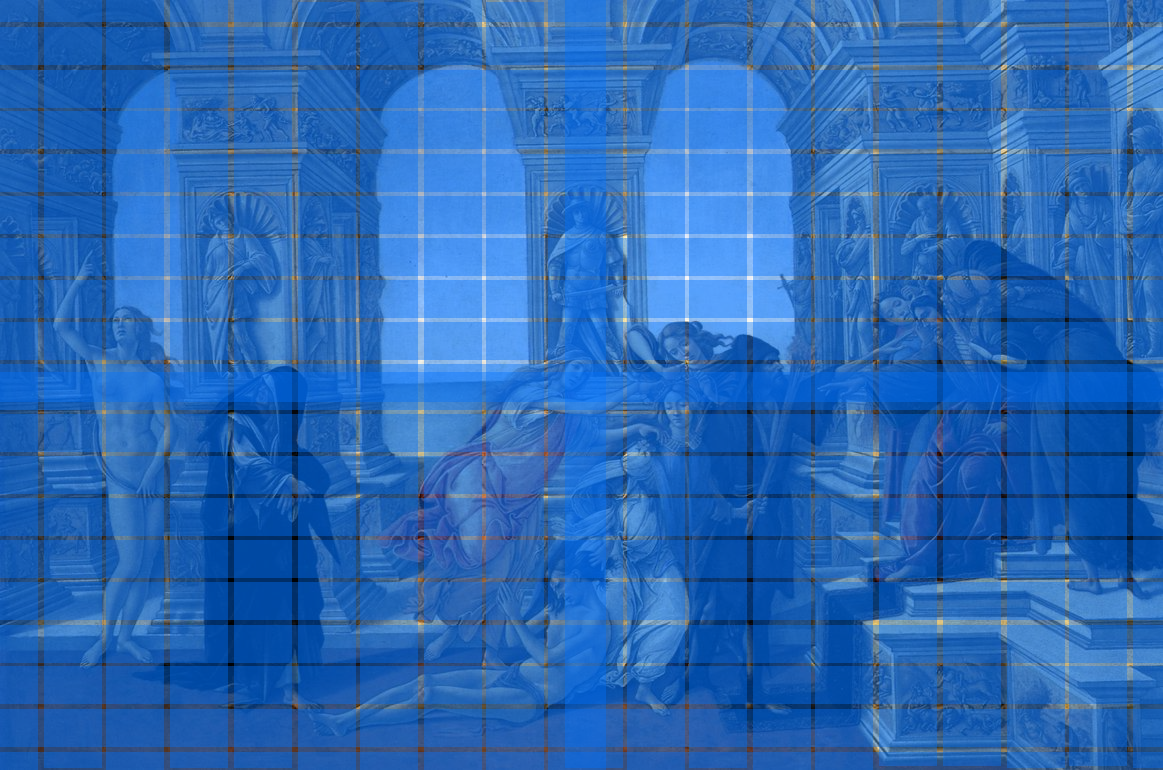
\includegraphics[width=1.00\textwidth]{billeder/koersel_snit}
    \end{center}
    }

\end{frame}

\end{document}
